\documentclass[aspectratio=169, table]{beamer}

\graphicspath{{../../images/}}
%\usepackage[beamertheme=./praditatheme]{Pradita}

\usetheme{Pradita}

\title{\Huge Model-View-* (MV*) Architecture\\\vspace{10pt}}
\subtitle{IF231303-Software Architecture}
\author{Alfa Yohannis}
\begin{document}

	\begin{frame}[plain]
		\maketitle
	\end{frame}

	\begin{frame}[fragile]
		\frametitle{Contents}
		
		\begin{columns}[t]
			\column{0.5\textwidth}
			\tableofcontents[sections={1-5}]
			
			\column{0.5\textwidth}
			\tableofcontents[sections={6}]
		\end{columns}
	\end{frame}

\section{Introduction to MV* Architectures}

\begin{frame}[fragile]{Introduction to MV* Architectures}
	\vspace{20pt}
	\textbf{Model-View-* (MV*)} is a set of architectures used in software development to separate business logic from the user interface. This approach aims to enhance separation of concerns, facilitate testing, and improve code readability and maintainability. \\
	The most common MV* variants include:
	\begin{itemize}
		\item \textbf{Model-View-Controller} (MVC): Divides responsibilities into Model (data and logic), View (user interface), and Controller (mediator between them).
		\item \textbf{Model-View-Presenter} (MVP): Emphasizes separation between presentation logic and View via a Presenter.
		\item \textbf{Model-View-ViewModel} (MVVM): Commonly used in data-binding-based development.
		\item \textbf{Model-View-Intent} (MVI): Frequently applied in reactive application development.
	\end{itemize}
\end{frame}

\begin{frame}[fragile]{Topics Covered in This Chapter}
	\vspace{20pt}
	This chapter discusses:
	\begin{itemize}
		\item Fundamental concepts of each Model-View-* architecture
		\item Key differences, advantages, and disadvantages
		\item Implementation across various technologies
		\item Practical examples of MV* application
	\end{itemize}
\end{frame}


\section{Model-View-Controller (MVC)}

\begin{frame}[fragile]{Introduction to MVC}
	\vspace{20pt}
	Model-View-Controller (MVC) is a software design pattern that separates an application into three main components to enhance modularity and maintainability.
\end{frame}

\begin{frame}[fragile]{Classic MVC Structure}
	\vspace{20pt}
	In a classic MVC implementation, the application is divided into three components:
	\begin{itemize}
		\item \textbf{Model}: Manages data, business logic, and application rules.
		\item \textbf{View}: Responsible for presenting data to the user.
		\item \textbf{Controller}: Connects Model and View, processes user input, and updates Model and View accordingly.
	\end{itemize}
\end{frame}

\begin{frame}[fragile]{Classic MVC Diagram}
	\vspace{20pt}
	\begin{figure}[h]
		\centering
		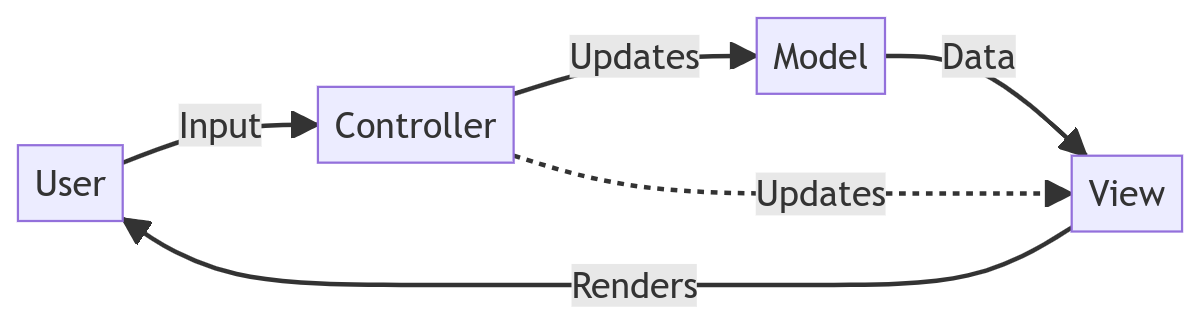
\includegraphics[width=\textwidth]{../images/mvc-classic.png}
		\caption{Classic MVC model when Users interact with controllers, not screens.}
		\label{fig:mvc-classic}
	\end{figure}
\end{frame}

\begin{frame}[fragile]{MVC in Modern Web/Desktop Frameworks}
	\vspace{20pt}
	Many modern web frameworks, such as Laravel, Django, and Spring, as well as desktop applications like JavaFX, adopt a slightly different MVC approach:
	\begin{itemize}
		\item The Controller often plays a more significant role, handling business logic and interactions with the Model.
		\item The View not only displays data but may also include programming code for dynamic rendering.
		\item The Model is frequently integrated with ORM (\textit{Object-Relational Mapping}) to facilitate database access.
	\end{itemize}
\end{frame}

\begin{frame}[fragile]{Modern MVC Diagram and Approach}
	\vspace{20pt}
	\begin{figure}[h]
		\centering
		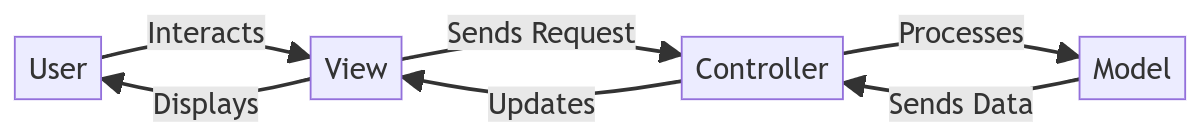
\includegraphics[width=\textwidth]{../images/mvc-modern.png}
		\caption{MVC in modern desktop/web frameworks.}
		\label{fig:mvc-modern}
			The modern framework approach enables better separation of business logic and user interface while integrating technologies like REST APIs and AJAX for more dynamic interactions.
	\end{figure}
\end{frame}

\section{Model-View-Presenter (MVP)}

\begin{frame}[fragile]{Introduction to MVP}
	\vspace{20pt}
	Model-View-Presenter (MVP) is a design pattern similar to MVC but with significant differences in component interactions. 
	MVP is commonly used in desktop applications or applications requiring greater control over UI and user interactions.
\end{frame}

\begin{frame}[fragile]{MVP Structure}
	\vspace{20pt}
	In an MVP implementation:
	\begin{itemize}
		\item \textbf{Model}: Handles business logic and data, interacting with databases and providing necessary data to the Presenter.
		\item \textbf{View}: Solely responsible for UI representation without business logic. It receives user input and forwards it to the Presenter, remaining passive.
		\item \textbf{Presenter}: Acts as a bridge between Model and View, processes input from View, interacts with Model, and updates View accordingly.
	\end{itemize}
\end{frame}

\begin{frame}[fragile]{MVP vs. Classic MVC}
	\vspace{20pt}
	Key differences between MVP and Classic MVC:
	\begin{itemize}
		\item In \textbf{MVP}, Presenter handles user input and displays data preparation and formatting logics, while Model plays a larger role handling business logics. The View only displays data and receives input without processing logic.
		\item In \textbf{MVC}, Controller also manages business logics, although the dominant role is still performed by Model, and connects Model and View, whereas View interacts directly with Controller.
		\item In \textbf{MVP}, View-Presenter communication is bidirectional, whereas in \textbf{MVC}, communication is more unidirectional.
	\end{itemize}
\end{frame}

\begin{frame}[fragile]{MVP Architecture Diagram}
	\vspace{20pt}
	\begin{figure}[h]
		\centering
		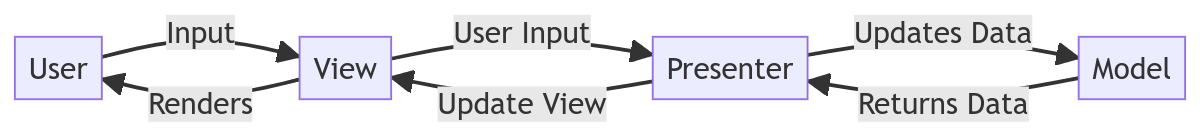
\includegraphics[width=\textwidth]{../images/mvp.png}
		\caption{Model-View-Presenter Architecture.}
		\label{fig:mvp-architecture}
	\end{figure}
\end{frame}

\begin{frame}[fragile]{Advantages of MVP}
	\vspace{20pt}
	The main advantages of MVP include:
	\begin{itemize}
		\item Clear separation of business logic and UI.
		\item Easier unit testing since Presenter can be tested independently of View.
	\end{itemize}
\end{frame}

\section{Model-View-ViewModel (MVVM)}

\begin{frame}[fragile]{Introduction to MVVM}
	\vspace{20pt}
	Model-View-ViewModel (MVVM) is a design pattern primarily used in desktop applications and platforms such as WPF (Windows Presentation Foundation) or other frameworks that support two-way data binding. MVVM separates presentation logic from the user interface in a highly structured manner.
\end{frame}

\begin{frame}[fragile]{MVVM Structure}
	\vspace{20pt}
	In an MVVM implementation:
	\begin{itemize}
		\item \textbf{Model}: Handles business logic and data. It interacts with databases or external services to provide necessary data to the ViewModel.
		\item \textbf{View}: Responsible for displaying the user interface and receiving user input. It focuses solely on rendering and does not manage logic or data.
		\item \textbf{ViewModel}: Acts as an intermediary between View and Model. It processes data received from the Model and makes it available in a form that the View can use. MVVM utilizes two-way data binding, ensuring automatic updates between View and ViewModel.
	\end{itemize}
\end{frame}

\begin{frame}[fragile]{MVVM vs. MVP}
	\vspace{20pt}
	The key differences between MVVM and MVP:
	\begin{itemize}
		\item In \textbf{MVVM}, the \textbf{ViewModel} prepares data from the Model for use in the View. It manages presentation logic and structures data for direct consumption by the View.
		\item In \textbf{MVP}, the \textbf{Presenter} handles input from the View, manages interactions with the Model, and updates the View, whereas the View only displays data without processing logic.
		\item MVVM enables \textbf{two-way data binding} between the View and ViewModel, ensuring automatic updates, while MVP follows a \textbf{one-way communication} model where the Presenter explicitly updates the View.
	\end{itemize}
\end{frame}

\begin{frame}[fragile]{MVVM Architecture Diagram}
	\vspace{20pt}
	\begin{figure}[h]
		\centering
		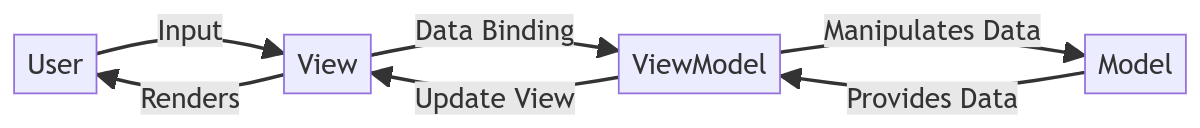
\includegraphics[width=\textwidth]{../images/mvvm.png}
		\caption{Model-View-ViewModel Architecture.}
		\label{fig:mvvm-architecture}
	\end{figure}
\end{frame}

\begin{frame}[fragile]{Advantages of MVVM}
	\vspace{20pt}
	The primary advantages of MVVM include:
	\begin{itemize}
		\item Clear separation of presentation logic from the user interface using two-way data binding.
		\item Easier testing and maintenance due to ViewModel handling all presentation logic.
		\item Simplified View structure, allowing it to focus solely on rendering.
	\end{itemize}
\end{frame}

\section{Model-View-Intent (MVI)}

\begin{frame}[fragile]{Introduction to MVI}
	\vspace{20pt}
	Model-View-Intent (MVI) is a design pattern commonly used in modern applications, particularly in Android development. 
	MVI aims to simplify data flow by providing a more declarative and reactive approach. 
	Each component in MVI has a distinct role in managing and manipulating application data.
\end{frame}

\begin{frame}[fragile]{MVI Structure}
	\vspace{20pt}
	In an MVI implementation:
	\begin{itemize}
		\item \textbf{Model}: Handles business logic and application data. It provides the application state that the View can observe and use.
		\item \textbf{View}: Responsible for displaying the user interface and receiving user input. It sends intents to the Presenter or ViewModel for processing and reacts to updates from the Model.
		\item \textbf{Intent}: Represents user actions or intentions, which are passed to the Presenter or ViewModel for processing. Intents describe what the user wants to do (e.g., pressing a button or selecting an item) and trigger changes in the application state.
	\end{itemize}
\end{frame}

\begin{frame}[fragile]{MVI vs. MVP}
	\vspace{20pt}
	Key differences between MVI and MVP:
	\begin{itemize}
		\item In \textbf{MVI}, \textbf{Intent} replaces direct user input handling, ensuring a more structured and reactive state management.
		\item In \textbf{MVP}, the \textbf{Presenter} manages presentation logic and processes input from the View to update the Model.
		\item MVI follows a \textbf{unidirectional data flow} where Intents are sent to the ViewModel or Presenter, which updates the Model and sends changes back to the View.
	\end{itemize}
\end{frame}

\begin{frame}[fragile]{MVI Architecture Diagram}
	\vspace{20pt}
	\begin{figure}[h]
		\centering
		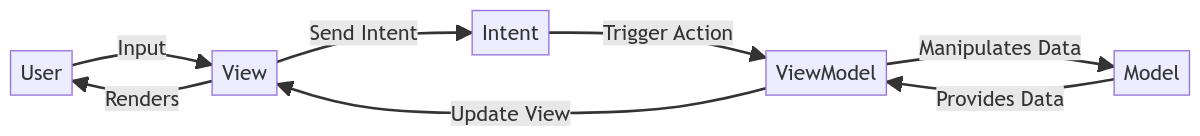
\includegraphics[width=\textwidth]{../images/mvi.png}
		\caption{Model-View-Intent Architecture.}
		\label{fig:mvi-architecture}
	\end{figure}
\end{frame}

\begin{frame}[fragile]{Advantages of MVI}
	\vspace{20pt}
	The primary advantages of MVI include:
	\begin{itemize}
		\item Simplified application state management.
		\item Improved reactivity and declarative data flow.
		\item Enhanced maintainability by reducing direct interactions between View and Model.
		\item A structured approach to handling application state and user interactions.
	\end{itemize}
\end{frame}

\section{Examples}

\begin{frame}[fragile]{Example Implementation}
	\vspace{20pt}
	This section presents an example implementation of software architecture using the Java programming language with the Java Swing library.
	
	The implementation includes:
	\begin{itemize}
		\item Two \texttt{JSpinner} components.
		\item A source \texttt{JSpinner} whose value change affects the target \texttt{JSpinner}.
		\item Processing of value changes according to the applied architecture.
	\end{itemize}
	
	Each architecture follows a distinct approach to handling \texttt{JSpinner} value changes:
	\begin{itemize}
		\item \textbf{Model-View-Controller (MVC)}: The controller acts as an intermediary, managing value updates between the View and Model.
		\item \textbf{Model-View-Presenter (MVP)}: The presenter takes over the intermediary role, handling logic for updating values.
	\end{itemize}
\end{frame}

\begin{frame}[fragile]{\LARGE{Architectural Variations and Sequence Diagrams}}
	\vspace{20pt}
	Additional variations of the architecture include:
	\begin{itemize}
		\item \textbf{Model-View-ViewModel (MVVM)}: Uses a binding mechanism to automatically synchronize changes between the View and Model.
		\item \textbf{Model-View-Intent (MVI)}: Utilizes intents to send changes from the View to the Model.
	\end{itemize}
	
	Each architecture is illustrated with a sequence diagram to show:
	\begin{itemize}
		\item Component interactions in handling \texttt{JSpinner} value changes.
		\item The data flow from the View to the Model.
		\item The process of updating values within the system.
	\end{itemize}
\end{frame}


\subsection{Model-View-Controller (MVC)}

\begin{frame}[fragile]{MVC Sequence Diagram}
	\vspace{20pt}
	\begin{figure}[h]
		\centering
		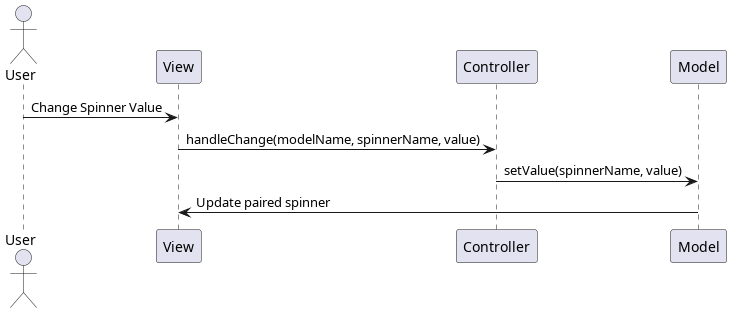
\includegraphics[width=\textwidth]{../images/out/mvc-sequence.png}
		\caption{Model-View-Sequence Architecture.}
		\label{fig:mvc-sequence}
	\end{figure}
\end{frame}

\begin{frame}[fragile]{MVC Interaction Flow}
	\vspace{20pt}
	This sequence diagram illustrates the interaction between the user, view, controller, and model in the Model-View-Controller (MVC) architecture.
	
	The interaction follows these steps:
	\begin{itemize}
		\item \textbf{User} changes the value in a graphical interface spinner.
		\item \textbf{View} captures the action and forwards it to the \textbf{Controller} via \texttt{handleChange()}.
		\item The method takes parameters such as:
		\begin{itemize}
			\item Model name.
			\item Spinner name.
			\item New value.
		\end{itemize}
	\end{itemize}
\end{frame}

\begin{frame}[fragile]{Controller as an Intermediary}
	\vspace{20pt}
	The controller manages interactions between the view and the model through the following steps:
	\begin{itemize}
		\item Receives the change request from the \textbf{View}.
		\item Calls \texttt{setValue()} on the \textbf{Model} to update the corresponding data.
		\item The model updates its internal data with the new value.
		\item Once updated, the model notifies the \textbf{View} to reflect the new value.
	\end{itemize}
\end{frame}

\begin{frame}[fragile]{Advantages of MVC}
	\vspace{20pt}
	In the MVC architecture:
	\begin{itemize}
		\item \textbf{Controller} manages user interactions and passes data to the model.
		\item \textbf{Model} stores and processes business logic and data changes.
		\item \textbf{View} strictly handles UI rendering without modifying business logic.
	\end{itemize}
	
	\textbf{Key benefits of MVC:}
	\begin{itemize}
		\item \textbf{Separation of Concerns}: Business logic is independent of UI, making maintenance easier.
		\item \textbf{Modularity}: Model and view can be updated or replaced without affecting other components.
		\item \textbf{Scalability}: Suitable for large applications requiring structured interaction between components.
	\end{itemize}
\end{frame}


\subsection{Model-View-Presenter (MVP)}

\begin{frame}[fragile]{MVP Sequence Diagram}
	\vspace{20pt}
	\begin{figure}[h]
		\centering
		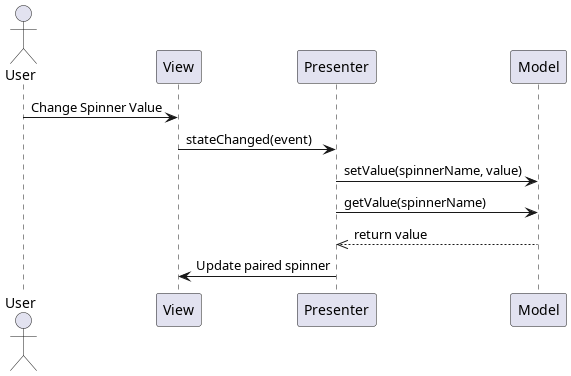
\includegraphics[width=.66\textwidth]{../images/out/mvp-sequence.png}
		\caption{Model-View-Presenter Sequence Architecture.}
		\label{fig:mvp-sequence}
	\end{figure}
\end{frame}

\begin{frame}[fragile]{MVP Interaction Flow}
	\vspace{20pt}
	This sequence diagram illustrates the interaction between the user, view, presenter, and model in the Model-View-Presenter (MVP) architecture.
	
	The interaction follows these steps:
	\begin{itemize}
		\item \textbf{User} changes the value in a graphical interface spinner.
		\item \textbf{View} captures the action and forwards it to the \textbf{Presenter} via \texttt{stateChanged()}.
	\end{itemize}
\end{frame}

\begin{frame}[fragile]{Presenter as an Intermediary}
	\vspace{20pt}
	The presenter acts as an intermediary between the view and the model, following these steps:
	\begin{itemize}
		\item Sends the new value to the \textbf{Model} via \texttt{setValue()}.
		\item Retrieves the updated value from the model via \texttt{getValue()}.
		\item The model returns the updated value to the presenter.
		\item The presenter updates the \textbf{View}, ensuring the UI reflects the new value.
	\end{itemize}
\end{frame}

\begin{frame}[fragile]{Advantages of MVP}
	\vspace{20pt}
	In the MVP architecture:
	\begin{itemize}
		\item \textbf{Presenter} handles all application logic and manages communication between the view and model.
		\item \textbf{View} only renders the UI without managing business logic or storing data.
	\end{itemize}
	
	\textbf{Key benefits of MVP:}
	\begin{itemize}
		\item \textbf{Separation of Concerns}: Presenter can be tested independently from the View.
		\item \textbf{Flexibility}: UI can be replaced without modifying the business logic inside the Presenter.
		\item \textbf{Maintainability}: Easier debugging and scalability due to clear responsibility separation.
	\end{itemize}
	
	This sequence diagram illustrates how MVP manages data flow and UI updates in a structured and efficient way.
\end{frame}


\subsection{Model-View-ViewModel (MVVM)}

\begin{frame}[fragile]{MVVM Sequence Diagram}
	\vspace{20pt}
	\begin{figure}[h]
		\centering
		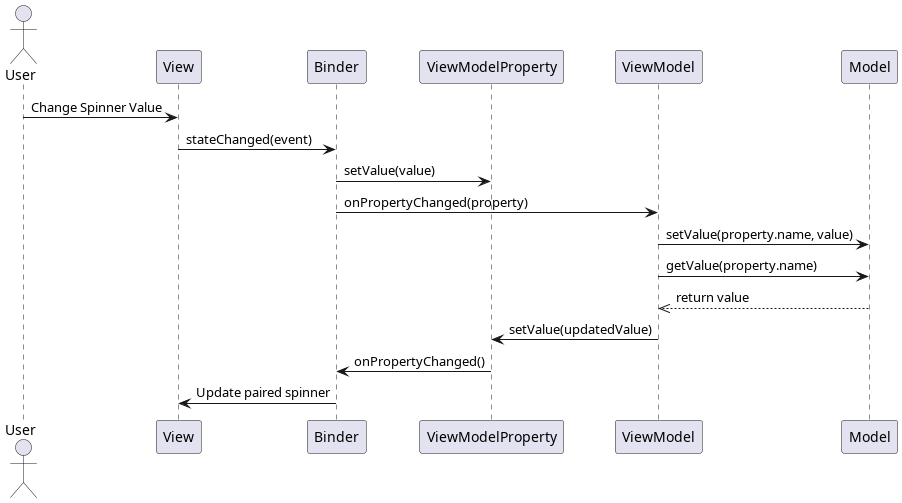
\includegraphics[width=.78\textwidth]{../images/out/mvvm-sequence.png}
		\caption{Model-View-ViewModel Sequence Architecture.}
		\label{fig:mvvm-sequence}
	\end{figure}
\end{frame}

\begin{frame}[fragile]{MVVM Interaction Flow}
	\vspace{20pt}
	This sequence diagram illustrates the interaction between the user, view, binder, ViewModelProperty, ViewModel, and model in the Model-View-ViewModel (MVVM) architecture.
	
	The interaction follows these steps:
	\begin{itemize}
		\item \textbf{User} changes the value in a graphical interface spinner.
		\item \textbf{View} captures the action and forwards it to the \textbf{Binder} via \texttt{stateChanged()}.
		\item The binder facilitates communication between the \textbf{ViewModelProperty} and the \textbf{ViewModel}.
	\end{itemize}
\end{frame}

\begin{frame}[fragile]{Data Synchronization in MVVM}
	\vspace{20pt}
	The binder ensures data synchronization between the view and model through the following steps:
	\begin{itemize}
		\item Updates \textbf{ViewModelProperty} via \texttt{setValue()}.
		\item Notifies the \textbf{ViewModel} of the change using \texttt{onPropertyChanged()}.
		\item ViewModel updates the \textbf{Model} via \texttt{setValue()}.
		\item Retrieves the latest value from the Model using \texttt{getValue()}.
		\item The Model returns the updated value to the ViewModel.
		\item ViewModel updates \textbf{ViewModelProperty} with the new value.
		\item ViewModelProperty notifies the \textbf{Binder} about the update via \texttt{onPropertyChanged()}.
		\item Finally, the binder updates the \textbf{View}, ensuring UI components reflect the updated value.
	\end{itemize}
\end{frame}

\begin{frame}[fragile]{Advantages of MVVM}
	\vspace{20pt}
	The MVVM architecture ensures that the view functions purely as a user interface without handling business logic. 
	The binder acts as a bridge between the View and ViewModel to ensure automatic data synchronization.
	
	\textbf{Key benefits of MVVM:}
	\begin{itemize}
		\item \textbf{Separation of Concerns}: Clear distinction between presentation and data layers.
		\item \textbf{Maintainability}: Easier code management and testing, as the ViewModel can be tested independently.
		\item \textbf{State Management}: Two-way data binding ensures UI and data remain synchronized.
	\end{itemize}
	
	This sequence diagram demonstrates how MVVM efficiently manages state changes, ensuring data consistency between the model and the view.
\end{frame}



\subsection{Model-View-Intent (MVI)}

\begin{frame}[fragile]{MVI Sequence Diagram}
	\vspace{20pt}
	\begin{figure}[h]
		\centering
		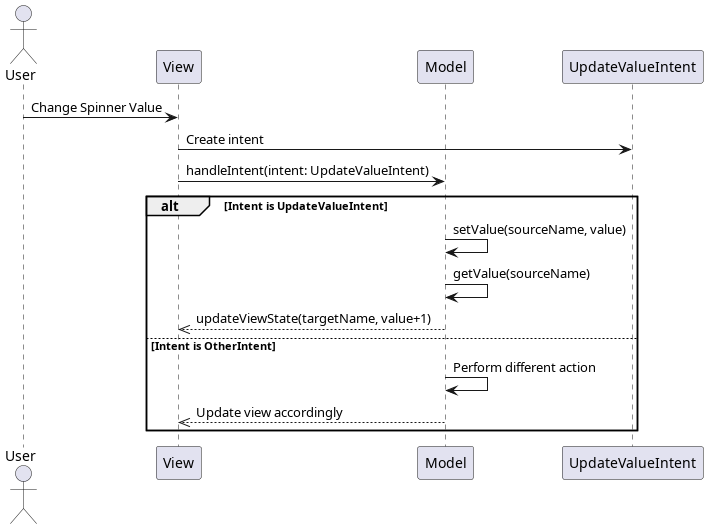
\includegraphics[width=.58\textwidth]{../images/out/mvi-sequence.png}
		\caption{Model-View-Intent Sequence Architecture.}
		\label{fig:mvi-sequence}
	\end{figure}
\end{frame}

\begin{frame}[fragile]{MVI Interaction Flow}
	\vspace{20pt}
	This sequence diagram illustrates the interaction between the user, view, model, and intent in the Model-View-Intent (MVI) architecture.
	
	The interaction follows these steps:
	\begin{itemize}
		\item \textbf{User} changes the value in a graphical interface spinner.
		\item \textbf{View} captures the action and creates an instance of \texttt{UpdateValueIntent}.
		\item The intent contains:
		\begin{itemize}
			\item The new value to be updated.
			\item The target component that will receive the new value.
		\end{itemize}
		\item The intent serves as a structured message instructing the model about the required changes.
	\end{itemize}
\end{frame}

\begin{frame}[fragile]{Intent Processing in MVI}
	\vspace{20pt}
	After the intent is created, the view calls the \texttt{handleIntent()} method on the \textbf{Model}, passing \texttt{UpdateValueIntent} as a parameter.
	
	The model processes the intent based on its type:
	\begin{itemize}
		\item \textbf{If the intent is \texttt{UpdateValueIntent}:}
		\begin{itemize}
			\item The model updates the corresponding value using \texttt{setValue()}.
			\item Retrieves the updated value using \texttt{getValue()}.
			\item Calls \texttt{updateViewState()} to update the UI with the new value.
		\end{itemize}
		\item \textbf{If the intent is another type (\texttt{OtherIntent}):}
		\begin{itemize}
			\item The model performs alternative processing, such as additional calculations or state changes.
			\item Updates the view accordingly.
		\end{itemize}
	\end{itemize}
\end{frame}

\begin{frame}[fragile]{Advantages of MVI}
	\vspace{20pt}
	This architecture ensures a clear separation of concerns between UI updates and business logic.
	
	\textbf{Key benefits of MVI:}
	\begin{itemize}
		\item \textbf{Maintainability}: Reduces direct dependencies between UI and business logic.
		\item \textbf{State Management}: Uses structured intent processing to manage application states.
		\item \textbf{Unidirectional Data Flow}: Reduces side effects and improves predictability.
	\end{itemize}
	
	This sequence diagram demonstrates how MVI enables a structured, predictable data flow while minimizing component dependencies.
\end{frame}


\end{document}
